% !TeX root = index.tex
%% Inside src/index.tex:

\documentclass{template}
\usepackage{graphicx,parskip,appendix,float}
\usepackage[ruled] {algorithm2e}
\usepackage{url,amsmath,amssymb,fancybox,listings,pdfpages,caption,multicol,datetime,rotating, booktabs}
%\usepackage[usenames,dvipsnames]{color}
\usepackage[pagebackref=false,pdffitwindow=true]{hyperref}
\usepackage{csquotes}
\usepackage{fontspec}
% \usepackage{xcolor}
% \usepackage{noto}
\usepackage{hyperref}
\usepackage[style=authoryear,backend=biber]{biblatex}
\usepackage{titlesec}% http://ctan.org/pkg/titlesec
% \usepackage{showframe}

% \setmainfont{Times New Roman}
% \setsansfont{Arial}
\setmonofont{JetBrainsMono}[
    Path=./assets/fonts/JBM/,
    Scale=0.85,
    Extension = .ttf,
    UprightFont=*-Regular,
    BoldFont=*-Bold,
    ItalicFont=*-Italic,
    BoldItalicFont=*-BoldItalic
    ]


\addbibresource{thesis.bib}

\hypersetup{
    pdftitle    = {},
    pdfauthor   = {},
    % pdfsubject  = {210657G},
    pdfkeywords = {enet, segnet, cnn},
    colorlinks  = true, anchorcolor = blue, filecolor = blue, urlcolor = blue,
    linkcolor   = colIdentifier,    %NOTE: change (blue) to (colIdentifier) to have links within the document in Black
    citecolor   = colIdentifier,    %NOTE: change (blue) to (colIdentifier) to have citation links within the document in Black
}

\definecolor{colBackGround}{rgb}{1,1,0.8}
\definecolor{colKeys}{rgb}{0,0,1}
\definecolor{colIdentifier}{rgb}{0,0,0}
\definecolor{colComments}{rgb}{0,.5,0}
\definecolor{colString}{rgb}{0,0,1}
\definecolor{colWhite}{rgb}{1,1,1}

\newcommand{\MyHookSign}{\hbox{\ensuremath\hookleftarrow}}

\newtheorem{Theorem}{Theorem}
\newtheorem{Proposition}[Theorem]{Proposition}
\newtheorem{Lemma}[Theorem]{Lemma}
\newtheorem{Proof}[Theorem]{Proof}
\newtheorem{Remark}[Theorem]{Remark}
\newtheorem{Claim}[Theorem]{Claim}
\newtheorem{Example}[Theorem]{Example}
\newtheorem{Definition}[Theorem]{Definition}

%NOTE: Setup for including program listings
\lstset{%
    float=H,
    basicstyle=\ttfamily,
    identifierstyle=\color{colIdentifier},
    keywordstyle=\color{colKeys}, %
    stringstyle=\color{colString},
    commentstyle=\color{colComments}, %
    % columns=flexible,
    columns=fullflexible,
    tabsize=2,
    % frame=single,
    framexleftmargin=5pt,
    framerule=0pt,
    frame=tb,
    extendedchars=true, %
    showspaces=false,
    showstringspaces=false,
    % numbers=left, %
    numberstyle=\footnotesize,
    breaklines=true,
    prebreak={\space\MyHookSign},
    language=Python,
    backgroundcolor=\color{colBackGround},
    breakautoindent=true, %
    captionpos=b%
} %\hypersetup{colorlinks=true, citecolor=\color{colIdentifier}}

\titleformat{\chapter}{\huge\bfseries}{\chaptername\ \thechapter}{0pt}{\vskip 10pt\raggedright}%
% Alter <after-sep> in the macro below to vary the separation after the \chapter title.
\titlespacing{\chapter}{0pt}{-20pt}{10pt}% \titlespacing{<command>}{<left>}{<before-sep>}{<after-sep>}[<right>]
\sloppy %NOTE: To ensure the Right Hand Margin is used (Especially for long URLS)
%NOTE: END of the document configuration settings

\begin{document}
\DeclareGraphicsExtensions{.jpg,.png,.gif,.pdf}
%NOTE: When inserting Figures if the extension of the graphic file is not provided LaTeX will automatically search
% for the extensions declared above, in the order declared.

\title{\huge{Software Design Document}}
\author{Thuvaragan S. 210657G \\ W.A.O Janandith 210234H}
\subtitle{Vision Based Robot Bin Picking Project, Sub Group ENet}
\modulecode{EN2160}
\modulename{Electronic Design Realization}
\degreetitle{Bachelor of Science in Engineering}
\rpttype{BSc Eng}
\principaladviser{Prof. Dr. Jayasinghe}
\beforeabstract
% 
% \prefacesection{Abstract}
% The Abstract of the report should be written here, it should provide a short summary of the work encompassing no more than 300 words.

% % \prefacesection{Acknowledgements}
% % The Acknowledgements section may be used to thank your supervisor, family, research funding bodies, or any other applicable individuals or institutions.

% \afterpreface 

\afterabstract
% \listofalgorithms   %NOTE: Will generate a list of Algorithms in the Table of Contents Section
% \lstlistoflistings  %NOTE: Will generate a list of Program Listings in the Table of Contents Section

%NOTE: Include the relative reference for each chapter to be included
% dividing the thesis file structure into a number of directories aids development
% format: directoryName/filename (the .tex extension is not required for the filename)

\chapter{Introduction}\label{ch:intro}
\pagenumbering{arabic} \setcounter{page}{1}
% \renewcommand*{\thesection}{\textbf{\alph{section}}}
% \renewcommand*{\thesubsection}{\roman{subsection}}
% \setcounter{section}{0}

% \section*{Introduction}

% \section*{Outline of the Solution}
% \renewcommand*{\thesubsection}{\alph{subsection}}
% \subsection{Requirement Analysis}
Image segmentation is a critical task in computer vision, enabling the partitioning of digital images into multiple segments to identify and delineate objects and regions of interest. This project aims to explore and implement practical techniques for efficient image segmentation, with a focus on leveraging deep learning models and state-of-the-art architectures.

The document outlines the research and development process undertaken to implement a robust image segmentation pipeline, encompassing background research, exploration of techniques, selection of frameworks and tools, and the initial setup for training and testing models.

\section{Background Research 1/3/2024}
There are two main types of image segmentation tasks: class segmentation and object segmentation. Class segmentation, also known as semantic segmentation, assigns semantic labels like "car" or "person" to each pixel in an image based on its class. This method is commonly used in applications such as autonomous driving and scene understanding. On the other hand, object segmentation, or instance segmentation, identifies and delineates individual objects within an image, assigning a unique mask to each object. Object segmentation is often utilized for tasks like tracking specific objects, such as in self-driving cars programmed to follow a particular vehicle.

\section{Exploring practical image segmentation techniques}
Efficiently implementing image segmentation involves crucial decision-making throughout the project life cycle. Some of the key factors that were found during the initial research are as follows,

\begin{enumerate}
  \item Choice of the deep learning framework: Pytorch or TensorFlow when it comes to python based frameworks.
  \item Choosing a good model architecture for the network design.
  \item Selecting an effective loss function to optimize and evaluate the model.
  \item Avoiding over-fitting and under-fitting.
  \item Evaluating the model's accuracy and efficiency comparatively.
\end{enumerate}

\section{Initial Setup 6/3/2024}
Properly setting up an environment for the model to training and testing is the hardest challenge in the implementation part. Various platforms such as \textbf{Kaggle}, \textbf{Deepnote}, \textbf{Pycharm} and \textbf{Datagrip} from JetBrains, and deep learning frameworks such as \textbf{TensorFlow}, \textbf{Pytorch}, \textbf{Caffe} and \textbf{Keras} were tried out as part of the exploration phase to decide on the compatibility of the setup with our project.

While platforms like Kaggle, Deepnote, PyCharm, and DataGrip from JetBrains offer valuable features, they were not chosen for our project due to various limitations. Kaggle and Deepnote, although providing cloud-based environments, often have restrictions on computational resources, limiting their suitability for training complex models like SegNet. PyCharm and DataGrip, on the other hand, are primarily used for local development, which can be computationally constrained for resource-intensive tasks. Additionally, these platforms may lack seamless integration with specific deep learning libraries required for our project.

Similarly, deep learning frameworks like TensorFlow, Caffe, and Keras were not selected due to their inherent characteristics. TensorFlow, while powerful, can be more complex and less intuitive for research and rapid prototyping compared to PyTorch. Caffe, although efficient, has a smaller community and limited support compared to more widely adopted frameworks. Keras, while user-friendly, is a high-level library built on top of other frameworks, which may introduce additional complexity and limitations for our specific requirements.

The following setup was decided as the way to test, the models we were assigned and the models we find moving forward on our research.

\begin{description}
  \item[Google Colab:] We opt to utilize Google Colab for implementing the models for training and testing due to several compelling reasons. Firstly, Google Colab provides a free and accessible cloud-based environment equipped with powerful GPUs, enabling faster model training compared to local machines, especially for computationally intensive tasks like image segmentation. Moreover, Colab offers seamless integration with popular deep learning libraries such as TensorFlow and PyTorch, simplifying the setup process and facilitating efficient implementation of complex models like SegNet. Additionally, Colab allows for collaborative work, enabling teams to share and collaborate on projects effortlessly. Its integration with Google Drive facilitates easy data access and storage, streamlining the entire workflow from data preparation to model evaluation. Overall, leveraging Google Colab for implementing the models ensures efficient, scalable, and collaborative model development for image segmentation tasks.

  \item[Pytorch:] PyTorch is a cutting-edge open-source deep learning framework designed for both research and production deployment. We selected Pytorch as the framework mostly due to following reasons,

        \begin{description}
          \item[Flexibility:] PyTorch is a flexible framework that allows you to create and train neural networks in a variety of ways. You can use pre-trained models, or you can create your own from scratch easily compared to other libraries.
          \item[Back-end support:] PyTorch supports multiple back-ends such as GPU/TPU hardware.
          \item[Domain libraries:] PyTorch has a rich set of domain libraries that make working with specific data verticals convenient. For example, for vision (image/video) related AI, PyTorch provides a builtin library called torchvision that we'll use extensively throughout this series.
          \item[Ease of use and community adoption:] PyTorch is an easy-to-use framework that is well-documented and has a large community of users and developers. Many researchers use PyTorch for their experiments, and the results in their published papers have an implementation of the model in PyTorch freely available.
        \end{description}
\end{description}
\chapter{SegNet}
\section{Introduction and Literary Review}
Segnet is a deep CNN model that has two distinct sections. The bottom section, also called an encoder, down-samples the input to generate features representative of the input. The top decoder section up-samples the features to create per-pixel classification. Each section is composed of a sequence of Conv-BN-ReLU blocks. These blocks also incorporate pooling or unpooling layers in down-sampling and up-sampling paths respectively. Below figure shows the arrangement of the layers in more detail. SegNet uses the pooling indices from the max-pooling operation in the encoder to determine which values to copy over during the max-unpooling operation in the decoder. While each element of an activation tensor is 4-bytes (32-bits), an offset within a 2x2 square can be stored using just 2-bits. This is more efficient in terms of memory used since these activations need to be stored while the model runs. [7]

\begin{figure}[H]
    \centering
    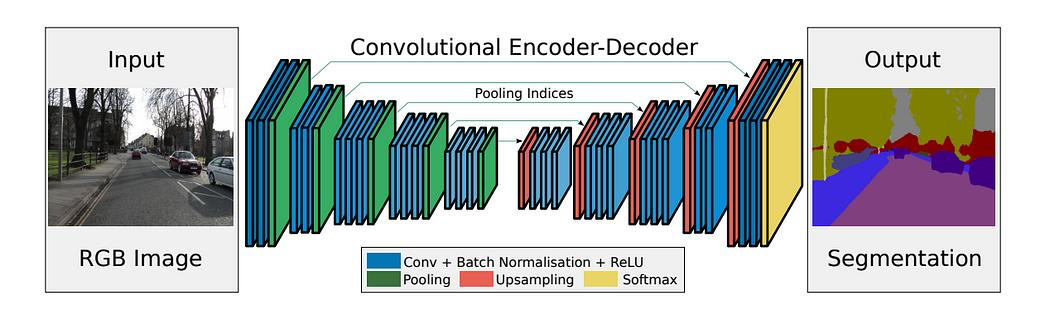
\includegraphics[width=450pt]{assets/segnet}
    \caption{SegNet Architecture Diagram}
    \label{fig:using:segnetarchi}
\end{figure}

\section{Implementation Trials 7/3/2024}
A pre-trained SegNet model [6] was tried to get setup in order to get to know the model implementations with SegNet. Here is a step-by-step process followed and the challenges faced along the way.

The Implementation was derived from an existing implementation found on the web.
% More details about the link....

First, the following libraries and packages were imported to the Google Colab environment.
\begin{lstlisting}
Cv2
Numpy
Pandas
Pickle
Tensorflow
\end{lstlisting}

After that dataset needed to be categorized as below to feed the dataset to the model without errors.
\begin{lstlisting}
data_path = 'Dataset/'

train_path = "Dataset/train/"
train_label_path = "Dataset/trainannot/"

valid_path = "Dataset/val/"
valid_label_path = "Dataset/valannot/"

test_path = "Dataset/test/"
test label. _path = "Dataset/testannot/"
\end{lstlisting}

During compilation, an error was found stating an indexing issue in Matplolib’s GridSpec to arrange a grid of subplot for visualizing image data.
\begin{lstlisting}
IndexError: index 0 is out of bounds for axis 0 with size 0
\end{lstlisting}

The error was fixed by having the random index generator to generate values starting from q1 instead of 0.

% TODO: What happened at implementing the default segnet model with the default dataset?

During the transition to a Roboflow dataset (more details in dataset chapter) the implementation of SegNet model by the subgroup was incompatible with the dataset generated by Roboflow and another obstacle was faced.

% \section{Key Takeaways}
% Implementing the SegNet model imposed several challenges due to the breaking changes in libraries and our lack of expertise in fixing some deeply rooted issues that required a more clear understanding of the libraries and the structure of the model.

% As the literature review of SegNet progressed, there were also explorations for other viable alternatives for SegNet by our team. During that process another better model called ENet was found and with the advice of the Supervisor, the project transitioned to testing ENet. This is discussed in more detail in the following chapters.

% Even though the current focus of the subgroup is ENet, a decision to keep reviewing the SegNet model and implementing it sometime was made to get more familiarity with the segmentation models.
\chapter{Dataset Preparation }
After evaluating the performance of pre-trained models, and with discussions with other subgroups, it became evident that training on a custom dataset tailored to our specific requirements was necessary. Consequently, we curated a dataset comprising images of boxes, which served as the foundation for training our image segmentation model.

\section{Roboflow Implementation Trials 10/3/2024}
We discovered a platform called Roboflow (\url{https://roboflow.com/}) that offers pre-trained datasets, streamlining the process of dataset preparation and integration. We leveraged one of their datasets specifically tailored for image segmentation tasks, comprising 333 images for training, 94 images for validation, and 48 images for testing. This particular dataset had been successfully utilized by other Roboflow users, yielding promising segmentation results, further reinforcing our decision to adopt it for our project.

\begin{figure}[H]
    \centering
    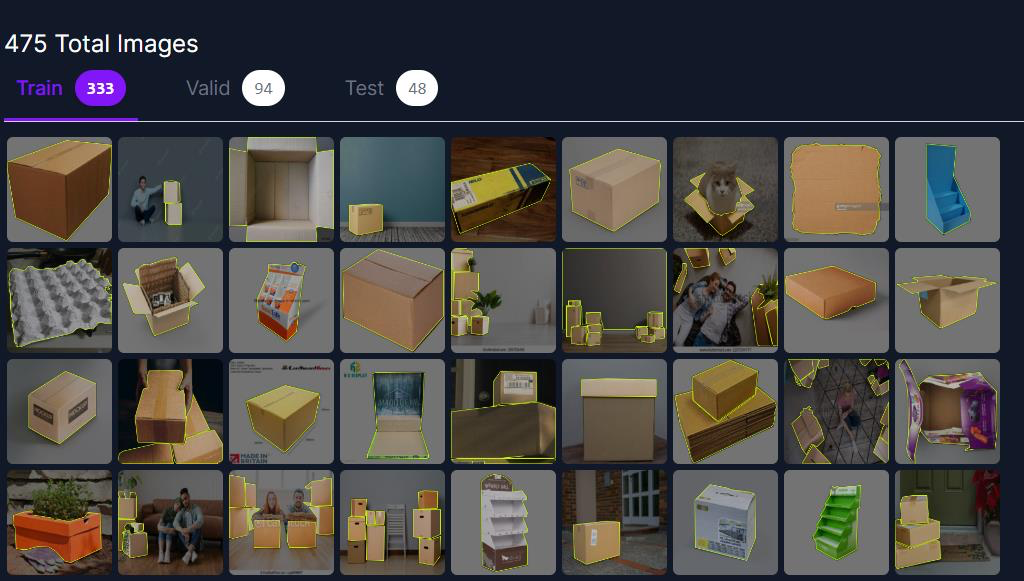
\includegraphics[width=450pt]{assets/roboflow}
    \caption{Roboflow Dataset Generation in Their Website}
    \label{fig:using:roboflowgen}
\end{figure}

Another reason why Roboflow was selected is it’s builtin interfaces for deploying in a Google Colab environment using a simple API call.

Here is how to port a Roboflow dataset in Google Colab:
\begin{lstlisting}[language=Python]
# 1.install the roboflow package
!pip install roboflow

# 2.dataset can be called
from roboflow import Roboflow
rf = Roboflow(api_key="########")
project = rf.workspace("vnudc").project("cardboard-boxes-vnal0")
version = project.version(1)
dataset = version.download("tensorflow")

# 3.use the dataset with your model
...
\end{lstlisting}

But when using this dataset to feed to the SegNet model we cam across this issue.

\begin{lstlisting}[language=bash]
TypeError: join() argument must be str, bytes, or os.PathLike object, 
not 'int'
\end{lstlisting}

We found out that this error is due to a mismatch of the format of the ported dataset with the format required by the model to split the dataset in to train , test and validate sets. We have to look into solve this error later.

\section{Self Curated Dataset 20/3/2024}
The dataset preparation phase is a critical component of the image segmentation pipeline, as the quality and diversity of the training data significantly influence the model's performance and generalization capabilities. In this regard, our expectations for the curated dataset encompass the following key aspects:

\subsection{Expectations}
\begin{description}
    \item[Representativeness]
          The dataset should be representative of the industrial scenarios and applications for which the image segmentation model is intended. It should capture a diverse range of object shapes, sizes, orientations, and backgrounds to ensure the model's robustness and ability to generalize effectively. This was achieved by hand picking the source images and using advanced ImageGen tools to generate variations of settings to speed up the collection process.

    \item[Annotation Quality]
          Accurate and consistent annotations are essential for training accurate segmentation models. The dataset should be meticulously annotated, with precise delineation of object boundaries and correct labeling of object classes. Since leveraging semi-automated annotation tools can contribute to maintaining high annotation quality, it was proposed as a viable method in a discussion. This was further expanded later to review many annotation tools in the web which are open-source.

    \item[Scalability]
          As the project progresses, the dataset should be easily scalable to accommodate additional data and annotations. This scalability will enable us to iteratively expand the dataset, thereby improving the model's performance and addressing potential biases or limitations identified during the training and evaluation phases. Review of literature material to achieve this is still undergoing.

    \item[Multi-model Compatibility]
          To facilitate comprehensive testing and bench-marking, the dataset should be compatible with multiple state-of-the-art image segmentation models and architectures. This compatibility will allow for comparative analyses and informed decision-making when selecting the most suitable model for our specific use case. With the initial discussion our subgroup decided to replicate the same features of the CamVid dataset, and then cross referencing with other subgroups lead to further literary review. Further Review to achieve this is still undergoing.

    \item[Common Mistake Mitigation]
          During the dataset creation process, it is essential to account for and mitigate common mistakes that can undermine the model's performance. These mistakes may include:
\end{description}

\begin{description}
    \item[Class Imbalance:] Ensuring a balanced distribution of object classes within the dataset is crucial to prevent the model from being biased toward dominant classes. This is achieved by simplifying the classes we wanted in our model to a lower number and focusing on finding the box first around the center. This might introduce some problems with navigation of the arm when cargo is uniquely positioned. Further review required.
    \item[Annotation Inconsistencies] Establishing clear annotation guidelines and conducting regular quality checks can help maintain consistency in the annotations across the dataset. All our subgroups decided to implement annotation as masks as it would allow for greater detail for certain models and can be simplified to a polygon if required later.
    \item[Data Leakage:] Proper dataset splitting and separation of training, validation, and test sets are necessary to prevent data leakage, which can lead to overly optimistic performance evaluations. We are tracking this problem in our goals, but since this is a problem that raises with scale and we are currently targeting a smaller database we decided to postpone this.
\end{description}

By addressing these expectations and proactively mitigating potential pitfalls, we aim to create a robust and versatile dataset that can serve as a solid foundation for training and evaluating our image segmentation models, ultimately contributing to the development of an efficient and accurate segmentation system.

\subsection{Implementation Trail}

% Many alternatives were looked upon and plans were made about the exact implementation of dataset with several brainstorming sessions within the subgroup and among the subgroups.
\chapter{ENet}
Later in our review of literature published related to segmentation models, we came across ENet (Efficient Neural Network), which is termed as a real-time semantic segmentation neural network designed for efficient processing on embedded systems and mobile devices. It was developed by researchers at Samsung AI Center and first presented in the paper "ENet: A Deep Neural Network Architecture for Real-Time Semantic Segmentation" published in 2016 [6].

Reviewing the research paper of ENet, it was found that performance wise and efficiency wise it is better than SegNet [5].

\begin{table}[h!]
    \centering
    \setlength{\arrayrulewidth}{0.5mm}
    \setlength{\tabcolsep}{18pt}
    \renewcommand{\arraystretch}{1.5}
    \begin{tabular}{ |p{1.5cm}|p{1.8cm}|p{1.8cm}|p{2cm}|p{2cm}| }
        % \hline
        % \multicolumn{5}{|c|}{Country List} \\
        \hline
        Network & 1024x512 & 1280x720 & Parameters & Model Size \\
        \hline
        ENet    & 20.4 ms  & 32.9 ms  & 0.36 M     & 1.5 MB     \\
        \hline
        SegNet  & 66.5 ms  & 114.3 ms & 29.4 M     & 117.8 MB   \\
        \hline
    \end{tabular}
    \caption{A comparison of computational time, number of parameters and model size required for ENet and SegNet [5]}
    \label{table:1}
\end{table}

The key advantages of ENet are its high speed, low computational requirements, and smaller memory footprint compared to existing models, while maintaining comparable accuracy. Considering the viability of the model for our project which mainly focuses on deploying a reliable model to identify boxes in an industrial environment, a suggestion was made at a discussion with the supervisor to consider this model, as it would allow us to deploy such a model in edge environments where memory and process is a constrained resource. The suggestion was reviewed and approved by the supervisor later and it lead to the transition from SegNet to ENet.

\subsection{Network Architecture}
The ENet architecture follows an encoder-decoder style topology with repeated modules of main and lateral branches. The encoder path captures higher-level semantics through a sequence of pooling and convolution operations, while the lateral connections preserve spatial information from earlier stages. The core building blocks are bottleneck modules with varying complexities [5]:

\begin{figure}[H]
    \begin{minipage}[t]{7.2cm}
        \begin{center}
            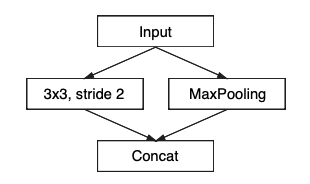
\includegraphics[width=200pt]{assets/enet/first.png}
            \caption{ENet initial block}
            \label{fig:using:enetinit}
        \end{center}
    \end{minipage}
    \hfill
    \begin{minipage}[t]{7.2cm}
        \begin{center}
            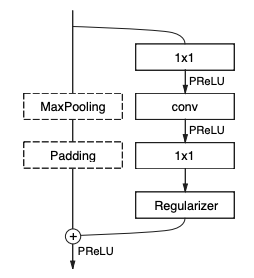
\includegraphics[width=200pt]{assets/enet/second.png}
            \caption{ENet bottleneck module}
            \label{fig:using:enetbottle}
        \end{center}
    \end{minipage}
\end{figure}

The following implementation in Pytorch achieves the network architecture provided by the paper [4]
\begin{description}
    \item[Initial Block:] Combines max-pooling and projection paths
    \item[Regular Bottleneck:] Applies identity mappings and 1x1 projections
    \item[Downsampling Bottleneck:] Reduces spatial dimensions with striding.
    \item[Dilated Bottleneck:] Employs dilated convolutions to expand receptive fields.
    \item[Upsampling Bottleneck:] Bilinear upsampling and fusion of encoder features.
\end{description}
This highly efficient architecture allows ENet to achieve real-time inference speeds while maintaining accuracy comparable to larger models like SegNet.

\section{Model Transition Plan 13/03/2024}
The following were planned to be acted on to create a model based on the original paper on ENet.
\begin{enumerate}
    \item Obtain the datasets mentioned in the paper (Cityscapes, CamVid, SUN RGB-D) and prepare them for training and testing.
    \item Implement the ENet architecture as described in the paper, including the encoder, decoder, and bottleneck modules. Using deep learning framework PyTorch
    \item Apply the design choices mentioned in the paper, such as early down-sampling, dilated convolutions, and Spatial Dropout.
    \item Train the ENet model on the datasets using the Adam optimization algorithm and the custom class weighing scheme described in the paper.
    \item Evaluate the trained model's performance on the test sets of the datasets, using metrics like class average accuracy, mean Intersection over Union (IoU), and inference time.
    \item Compare the results with existing models like SegNet, as done in the paper, and analyze the trade-offs between accuracy and processing time.
    \item Optionally, run the trained ENet model on embedded devices like the NVIDIA Jetson TX1 to assess its real-time performance and resource requirements.
\end{enumerate}

\section{ENet Paper Implementation 23/03/2024}
Paper implementation of ENet on CamVid dataset [4]. This guide assumes basic familiarity with notebooks and will include a brief setup process to get started with Google Colab.
\subsection*{Notebook Environment Setup: Google Colab}
\begin{enumerate}
    \item Go to \url{colab.research.google.com} -> File -> Open Notebook -> Search for the notebook from the Github Repo \url{https://github.com/CV-bin-picking/enet} and open it.
          \begin{figure}[H]
              \centering
              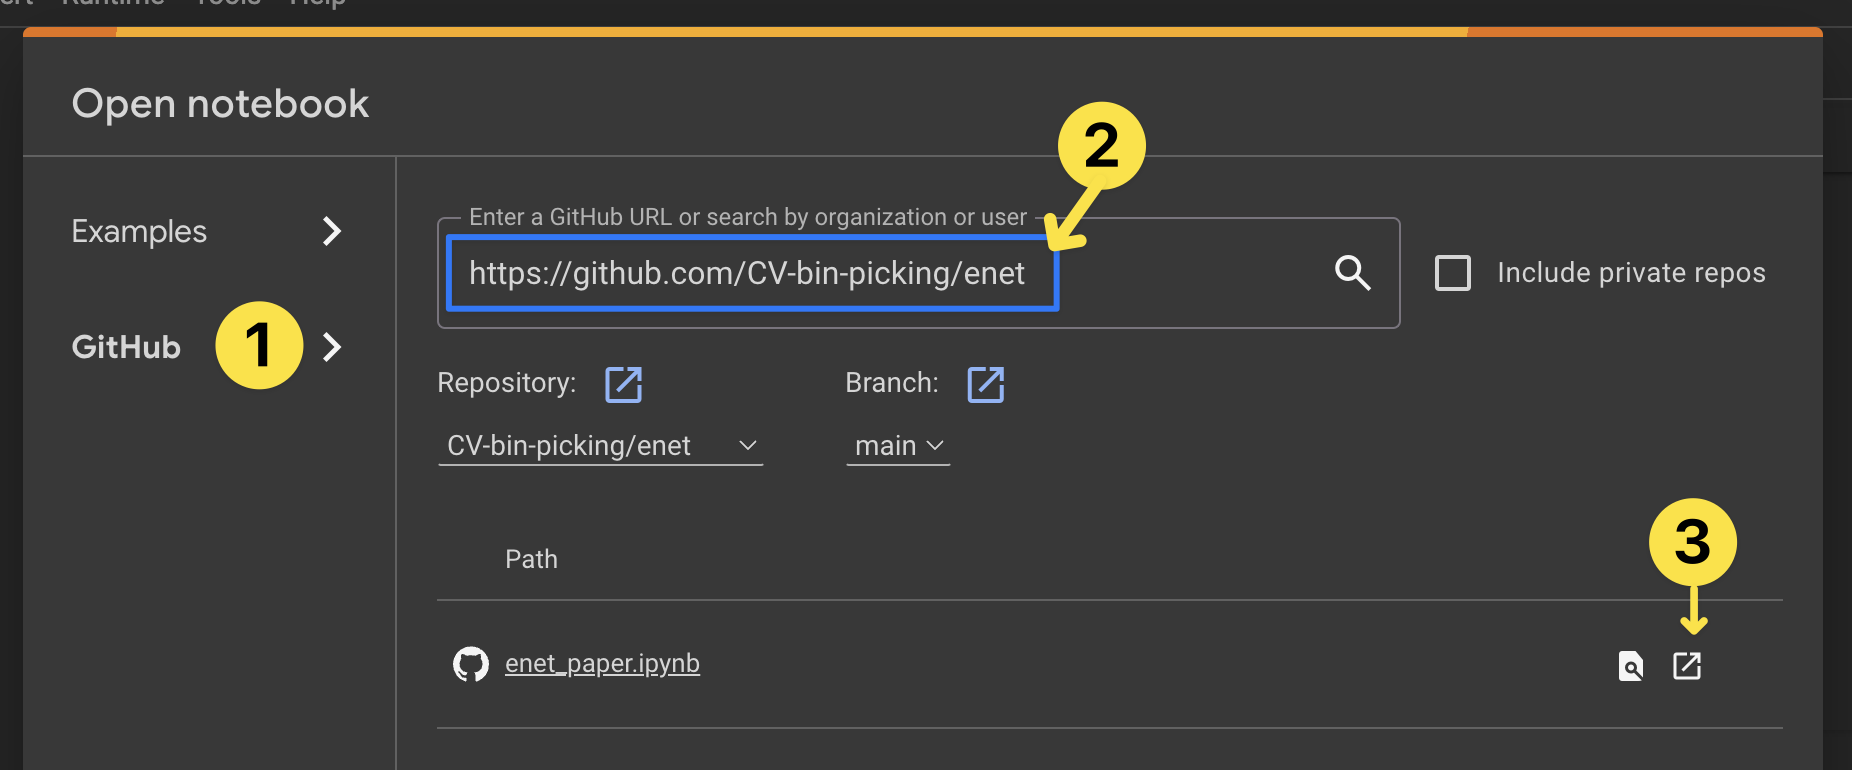
\includegraphics[width=450pt]{assets/enet/camvid/open.png}
              % \caption{SegNet Architecture Diagram}
              \label{fig:using:test1}
          \end{figure}
    \item Connect to GPU Runtime: In the menubar, go to Runtime -> Change runtime type. In the pop-up window, Runtime type as Python -> Select T4 GPU as the hardware accelerator -> Click Save.

          \textit{A Google Account is required. Colab interface is constantly changing, and it will autodetect recommended configurations for the notebook at launch. User is expected to do the best in either cases as GPU will improve the training time dramatically.}
    \item Importing dependencies: Execute the first cell in the notebook to prepare the python environment by importing required dependencies. \textit{You can ignore the warning about the notebook being not authored by Google after you've reviewed the source code}
          \begin{lstlisting}[language=Python]
import torch
import torch.nn as nn
import torch.nn.functional as F
import numpy as np
import matplotlib.pyplot as plt
from torch.optim.lr_scheduler import StepLR
import cv2
import os
from tqdm import tqdm
from PIL import Image
        \end{lstlisting}
    \item Configuring root directory: Change the root\_path variable string to "/content" before executing the second cell. This will configure the root directory where the model searches for the dataset and dumps the trained models. \textit{This step is allows the program to be executed in Colab as well as locally in your python environment with appropriate configuration.}
          \begin{lstlisting}[language=Python]
root_path = "/content" # change to `/content` for google colab
        \end{lstlisting}
    \item Configuring CamVid dataset: Uncomment the code in the third cell and execute it to download the CamVid dataset and extract it in the Colab root directory.
          \begin{lstlisting}[language=Python]
!wget https://www.dropbox.com/s/pxcz2wdz04zxocq/CamVid.zip?dl=1 -O CamVid.zip
!unzip CamVid.zip
        \end{lstlisting}
          \textit{This is initially commented to prevent accidentally downloading the CamVid dataset during bulk runs which might conflict with other datasets if you were to test them in the same notebook, which our subgroup is doing to transition to our own dataset}

\end{enumerate}
When the first three cells are successfully ran, the Google Colab environment is setup with the dataset and now we can create the network models.
\subsection*{ENet Model}
\textit{Full extend of the code is not presented here for the purpose of brevity, it is provided via the Github repo or the appendix}
\begin{enumerate}
    \item Creating the network blocks: Execute the next five cells to create the required architecture blocks proposed earlier for the network setup using Pytorch.
          \begin{lstlisting}[language=Python]
class InitialBlock(nn.Module):
    def __init__ (self,in_channels = 3,out_channels = 13):
        super().__init__()
        self.maxpool = nn.MaxPool2d(kernel_size=2,
                                      stride = 2,
                                      padding = 0)
        self.conv = nn.Conv2d(in_channels,
                                out_channels,
                                kernel_size = 3,
                                stride = 2,
                                padding = 1)
        self.prelu = nn.PReLU(16)
        self.batchnorm = nn.BatchNorm2d(out_channels)
        
    def forward(self, x):
        main = self.conv(x)
        main = self.batchnorm(main)
        side = self.maxpool(x)
        # concatenating on the channels axis
        x = torch.cat((main, side), dim=1)
        x = self.prelu(x)
        return x
        \end{lstlisting}
          \begin{lstlisting}[language=Python]
class UBNeck(nn.Module):
    def __init__(self, in_channels, out_channels, relu=False, projection_ratio=4):
        super().__init__()
        # Define class variables
        # Upsampling

    def forward(self, x, indices):
        x_copy = x
        # Side Branch
        # Main Branch
        # summing the main and side branches
        return x
        \end{lstlisting}
          \begin{lstlisting}[language=Python]
class RDDNeck(nn.Module):
    def __init__(self, dilation, in_channels, out_channels, down_flag, relu=False, projection_ratio=4, p=0.1):
        super().__init__()
        # Define class variables
        # calculating the number of reduced channels

    def forward(self, x):
        bs = x.size()[0]
        x_copy = x
        # Side Branch
        # Main Branch
        # Summing main and side branches
        x = x + x_copy
        x = self.prelu3(x)
        if self.down_flag:
            return x, indices
        else:
            return x
        \end{lstlisting}
          \begin{lstlisting}[language=Python]
class ASNeck(nn.Module):
    def __init__(self, in_channels, out_channels, projection_ratio=4):
    # Asymmetric bottleneck:
        super().__init__()
        # Define class variables

    def forward(self, x):
        bs = x.size()[0]
        x_copy = x
        # Side Branch
        # Main Branch
        # Summing main and side branches
        x = x + x_copy
        x = self.prelu3(x)
        return x
        \end{lstlisting}

          \begin{lstlisting}[language=Python]
class ENet(nn.Module):
    def __init__(self, C):
        super().__init__()
        # Define class variables
        self.C = C # number of classes
        # The initial block
        self.init = InitialBlock()
        # Five bottlenecks
        # Final ConvTranspose Layer

    def forward(self, x):
        # The initial block
        x = self.init(x)
        # Five bottlenecks
        # Final ConvTranspose Layer
        x = self.fullconv(x)
        return x
        \end{lstlisting}
    \item Instantiate the ENet model and attach Pytorch to GPU compute \textit{}
          \begin{lstlisting}[language=Python]
enet = ENet(12) # instantiate a 12 class ENet for CamVid
# logic to check and attach to gpu computes in different platforms
enet = enet.to(device)
        \end{lstlisting}
    \item Defining the loader
          \begin{lstlisting}[language=Python]
def loader(training_path, segmented_path, batch_size, h=320, w=1000):
    filenames_t = os.listdir(training_path)
    total_files_t = len(filenames_t)

    filenames_s = os.listdir(segmented_path)
    total_files_s = len(filenames_s)

    assert total_files_t == total_files_s

    if str(batch_size).lower() == "all":
        batch_size = total_files_s

    idx = 0
    while 1:
        # Choosing random indexes of images and labels
        batch_idxs = np.random.randint(0, total_files_s, batch_size)

        inputs = []
        labels = []

        for jj in batch_idxs:
            # Reading normalized photo
            img = plt.imread(training_path + filenames_t[jj])
            # Resizing using nearest neighbor method
            img = cv2.resize(img, (h, w), cv2.INTER_NEAREST)
            inputs.append(img)

            # Reading semantic image
            img = Image.open(segmented_path + filenames_s[jj])
            img = np.array(img)
            # Resizing using nearest neighbor method
            img = cv2.resize(img, (h, w), cv2.INTER_NEAREST)
            labels.append(img)

        inputs = np.stack(inputs, axis=2)
        # Changing image format to C x H x W
        inputs = torch.tensor(inputs).transpose(0, 2).transpose(1, 3)

        labels = torch.tensor(labels)

        yield inputs, labels
\end{lstlisting}
    \item Defining class weights
          \begin{lstlisting}[language=Python]
def get_class_weights(num_classes, c=1.02):
    pipe = loader(f"{root_path}/train/", f"{root_path}/trainannot/", batch_size="all")
    _, labels = next(pipe)
    all_labels = labels.flatten()
    each_class = np.bincount(all_labels, minlength=num_classes)
    prospensity_score = each_class / len(all_labels)
    class_weights = 1 / (np.log(c + prospensity_score))
    return class_weights


class_weights = get_class_weights(12)
\end{lstlisting}
    \item Defining hyper parameters
          \begin{lstlisting}[language=Python]
lr = 5e-4
batch_size = 10

criterion = nn.CrossEntropyLoss(weight=torch.FloatTensor(class_weights).to(device))
optimizer = torch.optim.Adam(enet.parameters(), lr=lr, weight_decay=2e-4)

print_every = 5
eval_every = 5
                        \end{lstlisting}
    \item Training Loop
          \begin{lstlisting}[language=Python]
train_losses = []
eval_losses = []

bc_train = 367 // batch_size  # mini_batch train
bc_eval = 101 // batch_size  # mini_batch validation

# Define pipeline objects
pipe = loader(f"{root_path}/train/", f"{root_path}/trainannot/", batch_size)
eval_pipe = loader(f"{root_path}/val/", f"{root_path}/valannot/", batch_size)

epochs = 100

# Train loop

for e in range(1, epochs + 1):
    train_loss = 0
    print("-" * 15, "Epoch %d" % e, "-" * 15)

    enet.train()

    for _ in tqdm(range(bc_train)):
        X_batch, mask_batch = next(pipe)

        # assign data to cpu/gpu
        X_batch, mask_batch = X_batch.to(device), mask_batch.to(device)

        optimizer.zero_grad()

        out = enet(X_batch.float())

        # loss calculation
        loss = criterion(out, mask_batch.long())
        # update weights
        loss.backward()
        optimizer.step()

        train_loss += loss.item()

    print()
    train_losses.append(train_loss)

    if (e + 1) % print_every == 0:
        print("Epoch {}/{}...".format(e, epochs), "Loss {:6f}".format(train_loss))

    if e % eval_every == 0:
        with torch.no_grad():
            enet.eval()

            eval_loss = 0

            # Validation loop
            for _ in tqdm(range(bc_eval)):
                inputs, labels = next(eval_pipe)

                inputs, labels = inputs.to(device), labels.to(device)

                out = enet(inputs)

                out = out.data.max(1)[1]

                eval_loss += (labels.long() - out.long()).sum()

            print()
            print("Loss {:6f}".format(eval_loss))

            eval_losses.append(eval_loss)

    if e % print_every == 0:
        checkpoint = {"epochs": e, "state_dict": enet.state_dict()}
        torch.save(
            checkpoint, "{}/ckpt-enet-{}-{}.pth".format(root_path, e, train_loss)
        )
        print("Model saved!")

print(
    "Epoch {}/{}...".format(e, epochs),
    "Total Mean Loss: {:6f}".format(sum(train_losses) / epochs),
)
                        \end{lstlisting}
          \textit{Training will take a long time even in Google Colab, with the free tier and adjusting to the loads, the current implementation in CamVid dataset runs for about 3 to 5 hours.}
\end{enumerate}
Executing the above cells will define the required Pytorch objects and dump the trained models in configured intervals into the root directory. You have the option to interrupt the training when you have obtained an iteration with satisfactory specifications to check it with the rest of the processes. This is useful for quickly changing certain parameters to evaluate the differences.

\subsection*{Infer using the model}
At the end of the training loop many ENet model files would've been dumped into the root folder. We can use the next infer code in the following way by renaming the variable name of the file to load according to the file name in the explorer or by doing vice versa. For example let's assume we want to load the model that is dumped during the 8th checkpoint (40th iteration).
\begin{figure}[H]
    \centering
    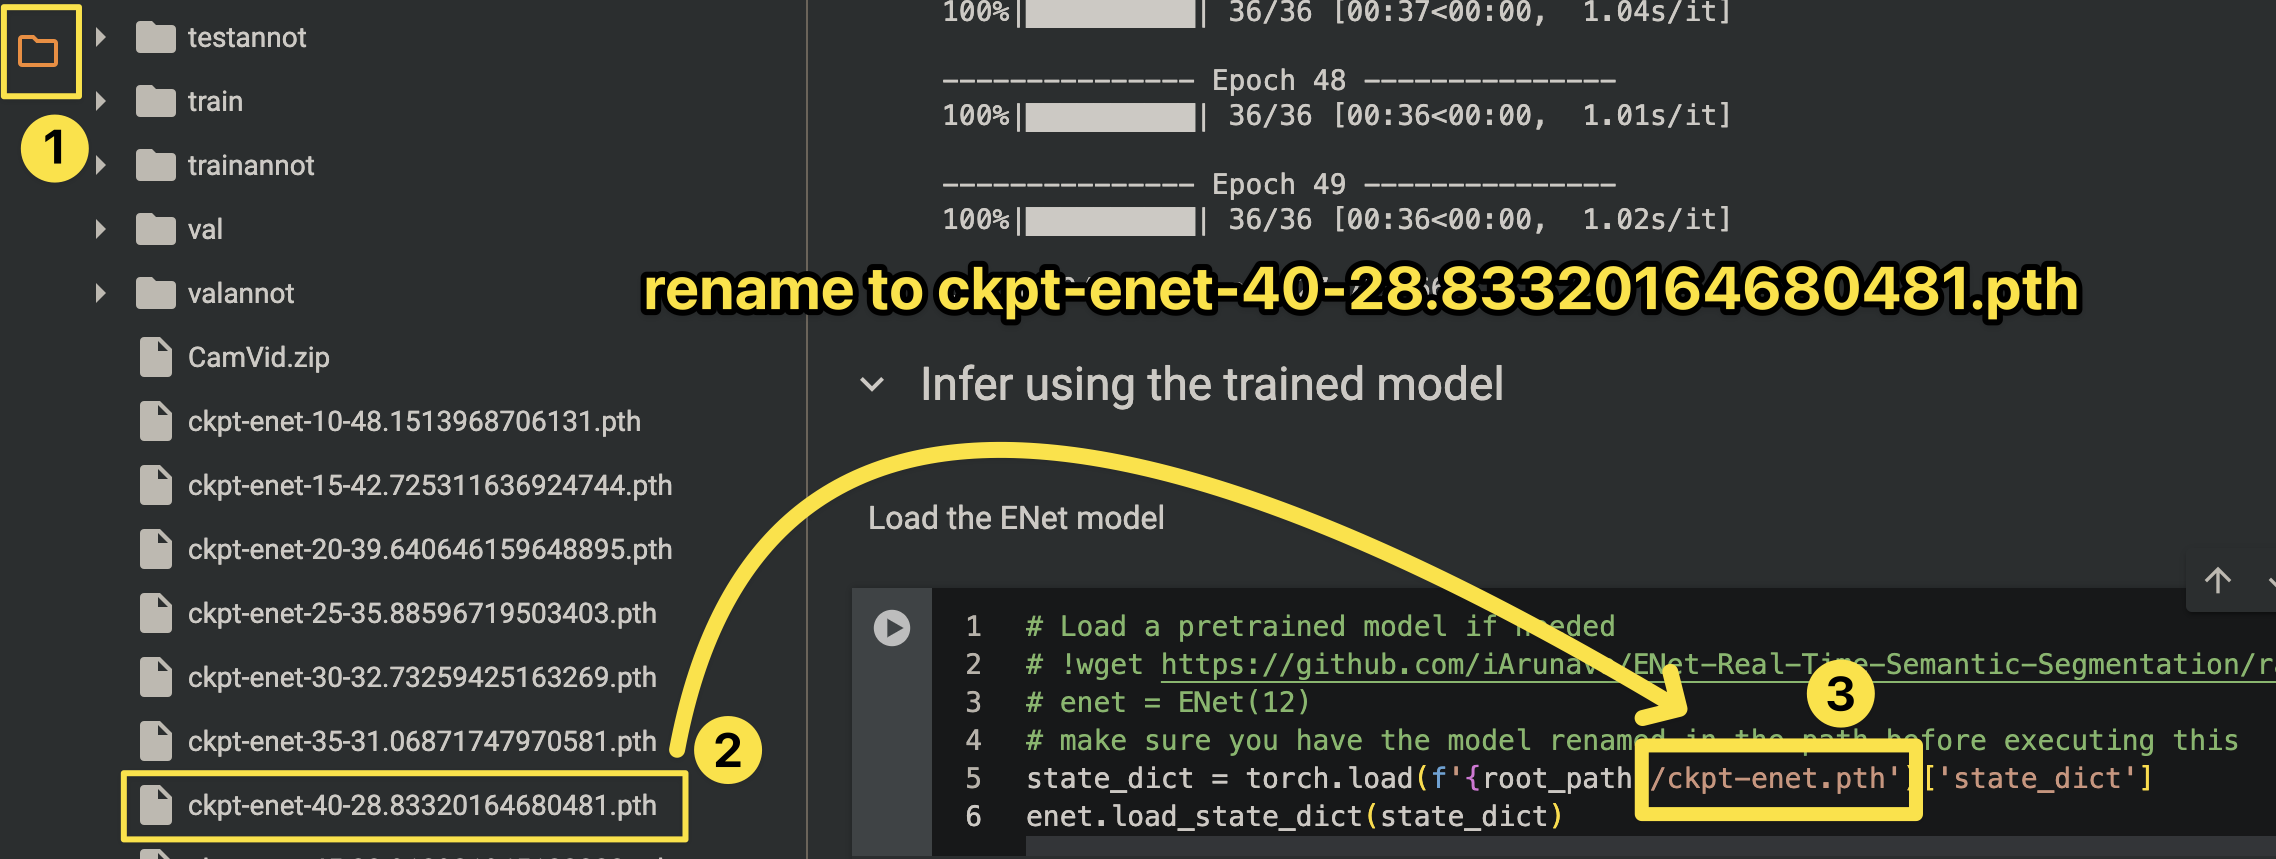
\includegraphics[width=450pt]{assets/enet/camvid/loadenet.png}
    % \caption{SegNet Architecture Diagram}
    \label{fig:using:test2}
\end{figure}

\subsection*{Testing on an image}
\begin{enumerate}
    \item Loading the image: Here you can change the "fname" variable to load the image file from your testing dataset. The code here has been filled with an existing image from the CamVid dataset.
          \begin{lstlisting}
fname = 'Seq05VD_f05100.png'
tmg_ = plt.imread(f'{root_path}/test/' + fname)
tmg_ = cv2.resize(tmg_, (512, 512), cv2.INTER_NEAREST)
tmg = torch.tensor(tmg_).unsqueeze(0).float()
tmg = tmg.transpose(2, 3).transpose(1, 2).to(device)
enet.to(device)
with torch.no_grad():
    out1 = enet(tmg.float()).squeeze(0)
\end{lstlisting}
    \item Generating the class label representation: Execute the following cells in the respective section to generate a label plot for the testing image
          \begin{lstlisting}
smg_ = Image.open(f'{root_path}/testannot/' + fname)
smg_ = cv2.resize(np.array(smg_), (512, 512), cv2.INTER_NEAREST)

mno = 8 # Should be between 0 - n-1 | where n is the number of classes

figure = plt.figure(figsize=(20, 10))
plt.subplot(1, 3, 1)
plt.title('Input Image')
plt.axis('off')
plt.imshow(tmg_)
plt.subplot(1, 3, 2)
plt.title('Output Image')
plt.axis('off')
plt.imshow(out2[mno, :, :])
plt.show()
\end{lstlisting}
          % The following are some of the outputs generated during testing.
          \begin{figure}[H]
              \centering
              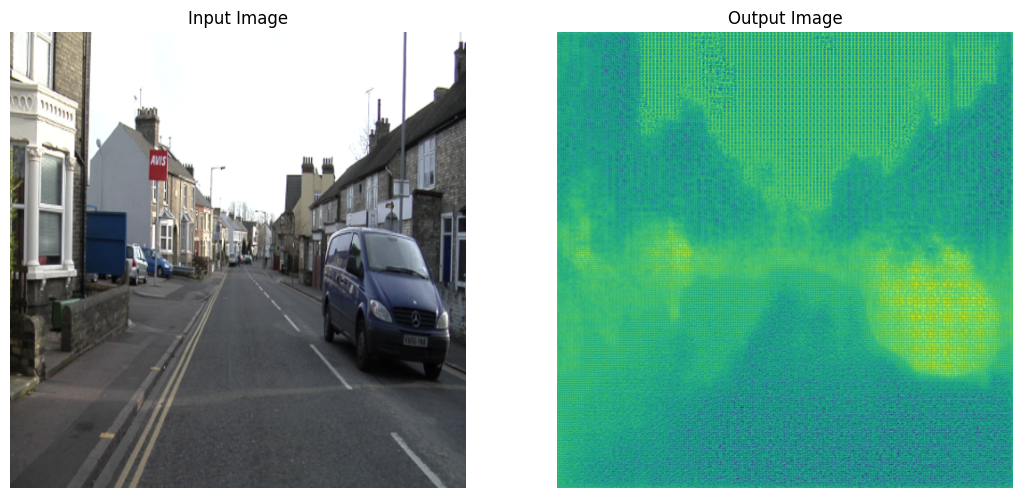
\includegraphics[width=450pt]{assets/enet/camvid/output1.png}
              \caption{Image segmentation was noticeable but far from perfect.}
              \label{fig:using:test5}
          \end{figure}
          \begin{figure}[H]
              \centering
              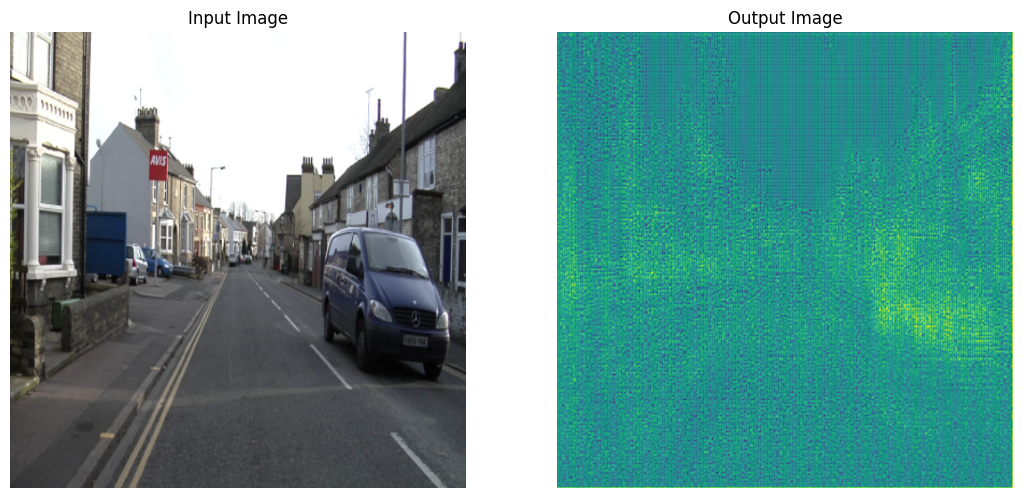
\includegraphics[width=450pt]{assets/enet/camvid/output1alt.png}
              \caption{Unexpected results during a testing stage done at a later date}
              \label{fig:using:test3}
          \end{figure}
    \item Color mapping and decoding: Executing the following code generates the segmented image and shows the ground truth which was already prepared to compare and observe the performance of the trained model.
          \begin{lstlisting}
b_ = out1.data.max(0)[1].cpu().numpy()

def decode_segmap(image):
    Sky = [128, 128, 128]
    Building = [128, 0, 0]
    Pole = [192, 192, 128]
    Road_marking = [255, 69, 0]
    Road = [128, 64, 128]
    Pavement = [60, 40, 222]
    Tree = [128, 128, 0]
    SignSymbol = [192, 128, 128]
    Fence = [64, 64, 128]
    Car = [64, 0, 128]
    Pedestrian = [64, 64, 0]
    Bicyclist = [0, 128, 192]

    label_colours = np.array([Sky, Building, Pole, Road_marking, Road,
                              Pavement, Tree, SignSymbol, Fence, Car,
                              Pedestrian, Bicyclist]).astype(np.uint8)
    r = np.zeros_like(image).astype(np.uint8)
    g = np.zeros_like(image).astype(np.uint8)
    b = np.zeros_like(image).astype(np.uint8)
    for l in range(0, 12):
        r[image == l] = label_colours[l, 0]
        g[image == l] = label_colours[l, 1]
        b[image == l] = label_colours[l, 2]

    rgb = np.zeros((image.shape[0], image.shape[1], 3)).astype(np.uint8)
    rgb[:, :, 0] = b
    rgb[:, :, 1] = g
    rgb[:, :, 2] = r
    return rgb

# decoding the images
true_seg = decode_segmap(smg_)
pred_seg = decode_segmap(b_)

figure = plt.figure(figsize=(20, 10))
plt.subplot(1, 3, 1)
plt.title('Input Image')
plt.axis('off')
plt.imshow(tmg_)
plt.subplot(1, 3, 2)
plt.title('Predicted Segmentation')
plt.axis('off')
plt.imshow(pred_seg)
plt.subplot(1, 3, 3)
plt.title('Ground Truth')
plt.axis('off')
plt.imshow(true_seg)
plt.show()
\end{lstlisting}
          % The following outputs were some samples from the testing done.
          \begin{figure}[H]
              \centering
              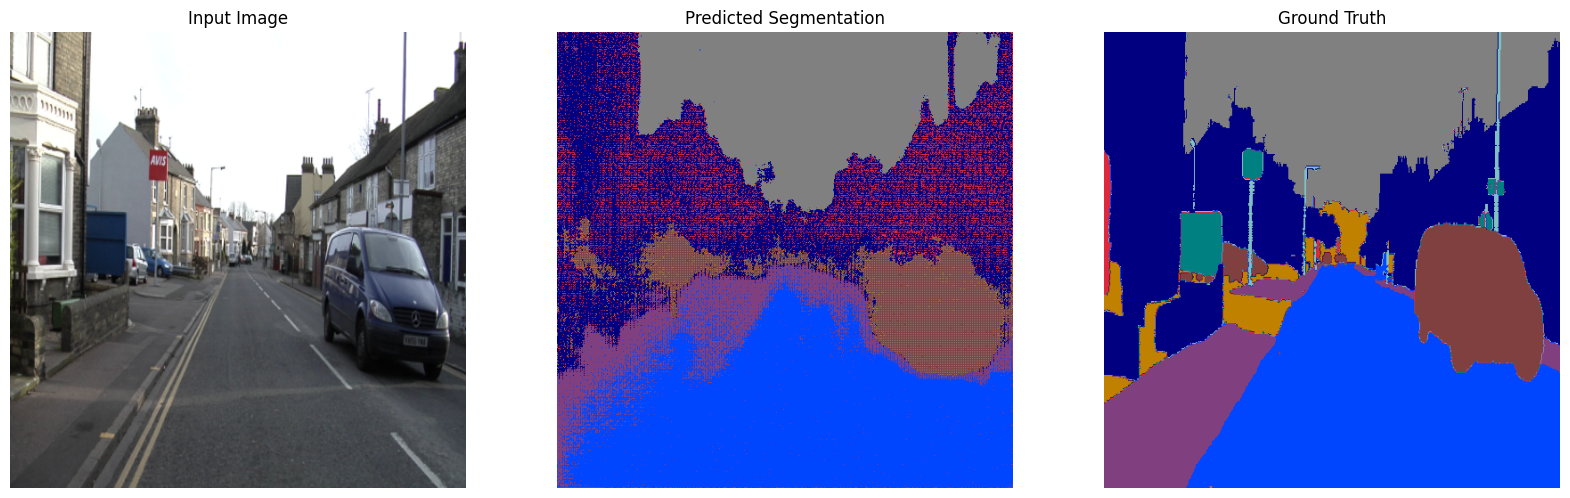
\includegraphics[width=450pt]{assets/enet/camvid/out1.png}
              \caption{The initial test results were promising after a training session with 100 iterations}
              \label{fig:using:test4}
          \end{figure}
          \begin{figure}[H]
              \centering
              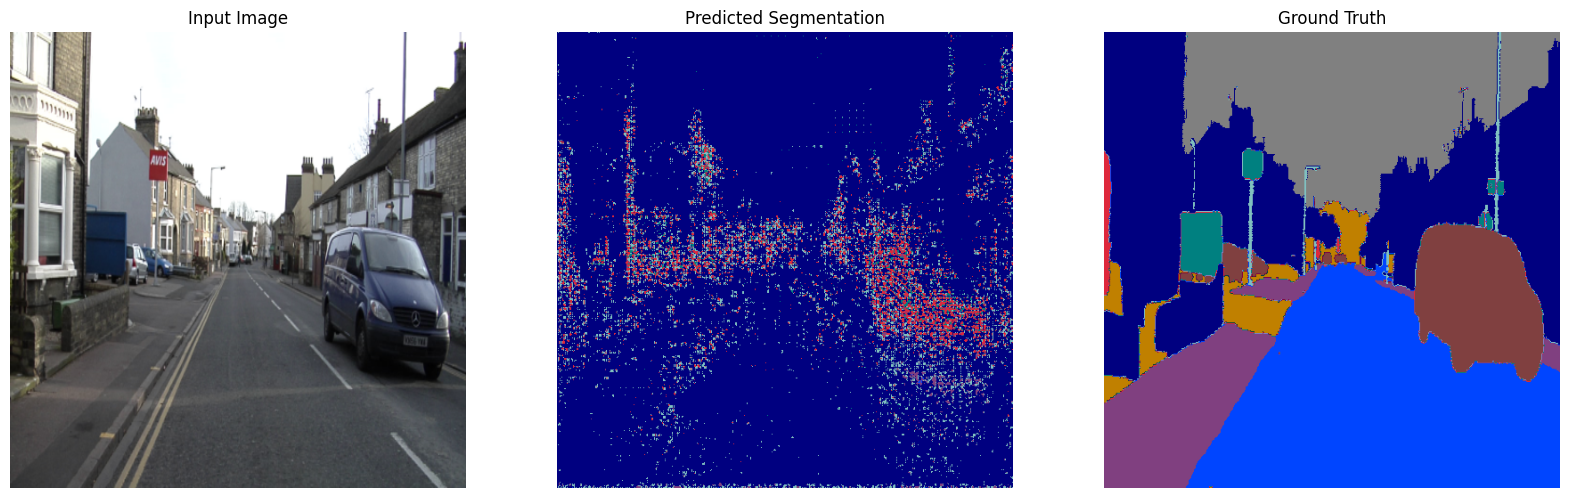
\includegraphics[width=450pt]{assets/enet/camvid/out1alt.png}
              \caption{The results were diminished in quality during another testing session with 100 iterations}
              \label{fig:using:test6}
          \end{figure}
\end{enumerate}



\subsection*{Saving the model and or checkpoints}
When there is a noticeable improvement observed, it is always a good idea to save the relevant parameters and model. The following code will help to save the relevant model to the root directory while also saving the parameter file in the Pytorch format which can then be used to do testing or for deployment or can be converted into a required format for improvement in other platforms. Any file in the Google Colab can be downloaded by navigating to the file directory as mentioned before and right clicking on the relevant file and clicking download.
\begin{lstlisting}
# Save the parameters
checkpoint = {
    'epochs' : e,
    'state_dict' : enet.state_dict()
}
torch.save(checkpoint, f'{root_path}/ckpt-enet-1.pth')
# Save the model
torch.save(enet, f'{root_path}/model.pt')
\end{lstlisting}

\subsection{Engineering Principles followed during the Implementation}
\begin{description}
    \item[Model Optimization:] The model leverages techniques like dimensionality reduction through bottleneck projections, parameter sharing through parallel dilated convolutions, and compact encoder-decoder topology to reduce computational complexity.
    \item[Hardware Acceleration:] By implementing the model in PyTorch and running it on Google Colab, we can take advantage of hardware acceleration through CUDA and cuDNN libraries on NVIDIA GPUs provided by Google's cloud infrastructure.
    \item[Data Parallelism:] The training loop is parallelized across multiple batches through PyTorch's DataLoader abstraction, enabling efficient utilization of the available GPU memory.
    \item[Checkpointing:] The training process supports periodic checkpointing of model weights, allowing training to be resumed from a saved state in case of interruptions or failures.
    \item[Modular Design:] The model implementation is structured into reusable components like bottleneck modules, making it easier to experiment with architectural variations or adapt the codebase for different tasks.
    \item[Visualization:] The notebook includes code for visualizing input images, ground truth segmentation masks, and model predictions, facilitating debugging and qualitative evaluation of results.
\end{description}

This implementation was possible within a short time because of the incredible work done on this existing Pytorch implementation [4] by user iArunava and the notebooks from Kaggle by ajax0564 [1], Davidtvs' repo on Pytorch implementation of ENet [3] were also referred to get more understanding.

With the initial steps completed successfully, we have achieved the first two objectives of obtaining the required datasets and implementing the ENet architecture faithfully in PyTorch. The subsequent goals involve training the model using the prescribed techniques, evaluating its performance against benchmarks, assessing inference speed on embedded hardware if viable, and ultimately comparing the results to existing models like SegNet. By methodically following the outlined plan, we aim to leverage ENet's computational efficiency to develop a reliable and lightweight semantic segmentation model tailored for deployment in resource-constrained industrial environments. Proceeding with the remaining objectives, we will meticulously train, optimize and validate the ENet implementation, culminating in a thorough analysis of its real-world applicability for our box identification task.
\chapter{Path Forward}
% The implementation of the most effective model for real-time semantic segmentation in our robot bin picking task has been a significant endeavor, combining theoretical knowledge from research literature with practical engineering principles. Throughout the project, we encountered several challenges and gained valuable insights, shaping our understanding of effective model development and deployment strategies.

\section{Pain Points}
One of the notable pain points encountered during the implementation process was the unpredictable nature of model performance during training. Despite following established methodologies and best practices, we observed instances where the trained models exhibited inconsistent results, sometimes performing better than expected, while other times yielding suboptimal outcomes. This variability underscored the inherent complexity of deep learning models and the sensitivity of their performance to various factors, such as hyperparameter tuning, data preprocessing, and random initialization.

Another challenge we faced was the integration of the ENet model with custom datasets. While the model architecture and implementation were well-documented, adapting it to work seamlessly with our specific dataset required careful consideration of data formats, preprocessing steps, and compatibility across different components of the pipeline. This process highlighted the importance of robust data handling and the need for modular, extensible implementations that can accommodate diverse data sources.

Additionally, we encountered issues related to computational resources and hardware limitations. Training deep learning models, especially for complex tasks like image segmentation, can be computationally intensive and often requires access to high-performance hardware accelerators. While leveraging Google Colab's GPU resources mitigated this challenge to some extent, we recognized the potential benefits of exploring more scalable and dedicated computing environments for larger-scale deployments.

\section{Upcoming}
Building upon the foundations established in this project, several avenues for future work and improvement have been identified and planned for the future weeks. It should be noted that as a subgroup our plan regarding the ENet implementation is already layed out in the relevant chapter, this section covers the overall goals of the project with our sub groups focus.
\subsection{Integration of Database Techniques 01/04/2024}
Exploring the integration of database techniques, such as those employed in the Segment Anything Model (SAM), into the ENet architecture could potentially enhance its performance and adaptability. By leveraging the strengths of both approaches, we aim to develop a more robust and versatile segmentation system.
\subsection{Utility Function Improvements 30/03/2024}
To streamline the training and evaluation processes, further enhancements to the utility functions within the ENet implementation are planned. These improvements will aim to improve reproducibility, facilitate hyperparameter tuning, and provide more comprehensive performance metrics and visualizations.
\subsection{Data Annotation and Preparation 01/04/2024}
Continuous efforts will be dedicated to annotating and preparing high-quality training and test data. This includes exploring semi-automated annotation techniques, crowdsourcing strategies within the group, and leveraging domain expertise to ensure accurate and diverse dataset representations.
% Literature Review and Model Integration: Ongoing literature reviews will be conducted to explore promising options for object detection convolutional neural networks (CNNs) and instance segmentation models. Integrating these advanced techniques with the ENet architecture, while preserving its computational efficiency advantages, is a key area of investigation.
\subsection{Modular Semantic Segmentation - Ongoing}
To enhance the versatility and adaptability of the system, efforts will be made to modularize the semantic segmentation component within the ENet pipeline. This modularization will allow for the seamless integration and evaluation of alternative semantic segmentation models, facilitating comparative analyses and informed decision-making based on performance and resource requirements.

\subsection{Instance Segmentation - 07/04/2024}
Integrate object identification models, such as Mask R-CNN or YOLACT, on top of the ENet-based semantic segmentation pipeline to create a comprehensive instance segmentation system. This involves enhancing the dataset diversity, exploring multi-task learning approaches, refining segmentation outputs with fusion techniques, optimizing for edge deployment, ensuring continuous training, and planning for real-world integration and deployment.

\subsection{Deterministic Environments and Reproducibility - Ongoing}
Exploring deterministic environments such as Nix or Docker will be a priority to ensure strict reproducibility of models and results across different platforms and computing environments. This will contribute to the overall robustness and reliability of the developed solutions.
\subsection{Edge Deployment and Docker Setup - TBD}
As the project progresses, a focus will be placed on streamlining the deployment process for running trained models on edge devices and embedded systems. This will involve establishing a Docker-based deployment setup, enabling efficient and consistent execution of the models in real-world scenarios.

By addressing these future directions, we aim to continuously improve the performance, flexibility, and real-world applicability of the ENet-based image segmentation system, contributing to the advancement of computer vision techniques and their practical applications across various domains.

\chapter*{References}

 [1] ajax0564, “E-NET image segmentation,” Kaggle, https://www.kaggle.com/code/ajax0564/e-net-image-segmentation (accessed Mar. 28, 2024).

   [2] A. Shamsian, "Image segmentation overview \& enet implementation," Medium,https://medium.com/@mista2311/image-segmentation-overview-enet-implementation-8394ff71cf26 (accessed Mar. 28, 2024).

   [3] Davidtvs, “Davidtvs/Pytorch-ENet: Pytorch implementation of enet,” GitHub,https://github.com/davidtvs/PyTorch-ENet?tab=readme-ov-file (accessed Mar. 28, 2024).

   [4] iArunava, “IARUNAVA/Enet-real-time-semantic-segmentation: Enet - a neural net architecture for real time semantic segmentation,” GitHub, https://github.com/iArunava/ENet-Real-Time-Semantic-Segmentation (accessed Mar. 28, 2024).

   [5] A. Paszke, A. Chaurasia, S. Kim, and E. Culurciello, “Enet: A deep neural network architecture for real-time semantic segmentation,” arXiv.org, https://arxiv.org/abs/1606.02147 (accessed Mar. 28, 2024).

   [6] Kulkarnikeerti, “Kulkarnikeerti/segnet-semantic-segmentation: Deep convolutional encoder-decoder network for image segmentation,” GitHub, https://github.com/kulkarnikeerti/SegNet-Semantic-Segmentation (accessed Mar. 28,2024).

   [7] V. Badrinarayanan, A. Kendall, and R. Cipolla, “SegNet: A deep convolutional encoder-decoder architecture for image segmentation,” IEEE Transactions on Pattern Analysis and Machine Intelligence, vol. 39, no. 12, pp. 2481-2495, Dec. 2017.doi:10.1109/tpami.2016.2644615

\footnotesize  %NOTE: reduced the size of the text for the bibliography
%NOTE: set the style for the bibliography and display the references used within the document
\printbibliography
\normalsize
\appendix
% \chapter{Project Specification}
% Summary of the project outline.

% \section{Functional Requirements}
% some text here

% \section{Non-Functional Requirements}
% some text here

% \chapter{Project Management}
% Discussion on how the project was managed. What things impacted the success of the project. How does the continually revised versions of the project plan compare to the initial draft developed at the start of the project. Did everything run according the schedule. Did elements such as exams \& coursework have any impact. 

% \chapter{Another Appendix}

% This appendix makes use of the \emph{rotating} package to rotate both figures and tables ninety degrees allowing for large datasets and illustrations to be represented.

% \begin{sidewaystable}
% \begin{center}
%    \begin{tabular}{llllllllll} 
%    \toprule
%    \textbf{Heading 1} & \textbf{Heading 2}  & \textbf{Heading 3}  & \textbf{Heading 4}  & \textbf{Heading 5}  & \textbf{Heading 6}  & \textbf{Heading 7}  & \textbf{Heading 8}  & \textbf{Heading 9}  & \textbf{Heading 10}  \cr
%    \midrule
%    aaa & bbbb & cccc & dddd & eeee & ffff & gggg & hhhh & iiii & jjjj \cr 
%    aaa & bbbb & cccc & dddd & eeee & ffff & gggg & hhhh & iiii & jjjj \cr 
%    aaa & bbbb & cccc & dddd & eeee & ffff & gggg & hhhh & iiii & jjjj \cr 
%    aaa & bbbb & cccc & dddd & eeee & ffff & gggg & hhhh & iiii & jjjj \cr 
%    aaa & bbbb & cccc & dddd & eeee & ffff & gggg & hhhh & iiii & jjjj \cr 
%    aaa & bbbb & cccc & dddd & eeee & ffff & gggg & hhhh & iiii & jjjj \cr 
%    \bottomrule
%    \end{tabular}
% \caption[A Short Caption for the table]{
% 	A much longer caption that will not be listed in the list of tables page.
% }
% \label{tab:sidewaysTable}
% \end{center}
% \end{sidewaystable}

% \begin{sidewaysfigure}
% \centerline{\includegraphics[width=7in]{appendix/images/samplepng}}
% \caption[A Sideways Figure]{
% 	A much longer caption that will not be listed in the list of figures page.
% }
% \label{fig:sidewaysFigure}
% \end{sidewaysfigure}

% \chapter{Presentation Slides}

% The slides from the formal presentation should be provided here in not more than two pages. 

% \chapter{Project Log}

% The following is a weekly summary of the work carried during the development of this body of work. It covers tasks that were completed, tutorials that were worked through, articles that were read and reviews of discussions / meetings held with the project supervisor and other third parties. 

% \section*{Week Beginning: Monday 27/09/2010}

% First week working on the project. Had a meeting with supervisor and discussed some of the issues related to the project. The first deliverable is due for the end of next week (project outline \& ethics form). 

% \begin{itemize}
%   \item Downloaded and Installed \LaTeX \space (MikTeX full install), Ghostscript, Ghostview \& Winshell. 
%   \item Started to get to grips with the \LaTeX \space system by making simple modifications to the template and editing the project log.
%   \item Developed a Mind Map to clarify understanding of project elements.
%   \item Prepared an initial draft of project plan in the form of a Gantt chart. 
%   \item Prepared and revised 1 page draft of project summary \& filled in ethics form. 
% \end{itemize}




\end{document} %NOTE: END of document, nothing after this point% This is the beginning.